% Created 2021-12-23 Thu 17:15
% Intended LaTeX compiler: pdflatex
\documentclass[11pt]{article}
\usepackage[utf8]{inputenc}
\usepackage[T1]{fontenc}
\usepackage{graphicx}
\usepackage{grffile}
\usepackage{longtable}
\usepackage{wrapfig}
\usepackage{rotating}
\usepackage[normalem]{ulem}
\usepackage{amsmath}
\usepackage{textcomp}
\usepackage{amssymb}
\usepackage{capt-of}
\usepackage{hyperref}
\author{Abhijit Paul}
\date{\today}
\title{}
\hypersetup{
 pdfauthor={Abhijit Paul},
 pdftitle={},
 pdfkeywords={},
 pdfsubject={},
 pdfcreator={Emacs 27.1 (Org mode 9.3)}, 
 pdflang={English}}
\begin{document}

\tableofcontents


\section*{Crash Courses}
\label{sec:orge15ca35}
\href{https://www.youtube.com/watch?v=tpIctyqH29Q\&list=PLH2l6uzC4UEW0s7-KewFLBC1D0l6XRfye\&index=1}{Playlist}\\
\subsection*{Computer Science}
\label{sec:org885a613}
\subsubsection*{Ep 1}
\label{sec:org8c374aa}
This course covers -\\
\begin{itemize}
\item History\\
\item Philosophy\\
\end{itemize}
\subsubsection*{Ep 2: Early Computing}
\label{sec:org61ba15a}
Abacus is used for \texttt{counting}. Like if we had a queue of 1236 people and we have to count them, its cumbersome to do that by hands. So we use Abacus to count the people one by one. The following example show how to count 1251 using abacus.\\
1251 = 1000 + 2*100 + 5*10 + 1\\
 \begin{center}
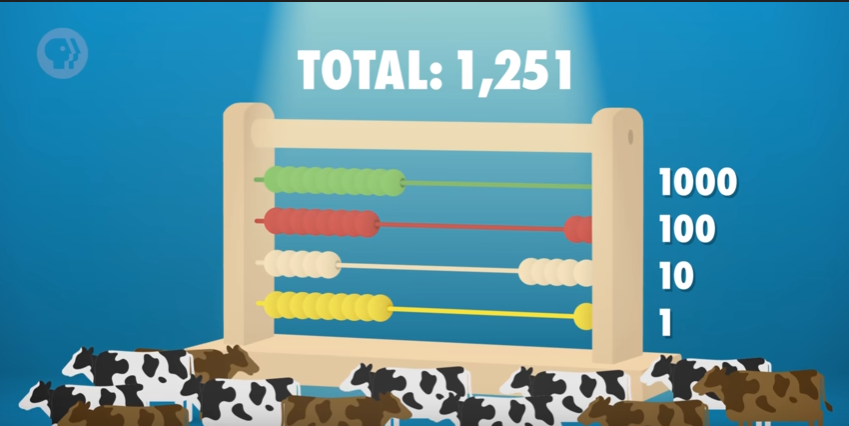
\includegraphics[width=.9\linewidth]{./abacus.png}
\end{center}

At first, during 1500-1700s, the counting was done through hands, by people. Ironically, it was a job position and the people of that job were called \texttt{Computers}, as in - people who compute.\\

Liebniz invented a addition machine in 1694 and commented, "Its beyond the dignity of great man to do computaion when a mere peasant can do that faster with the aid of a machine." Many machines of such kind were invented but they worked in a particular manner. They are known as mechanical calculator.\\
\href{https://www.youtube.com/watch?v=3h71HAJWnVU}{Mechanical Calculator - how do they work?}\\

You see, subtraction(using 9's complement), multiplication(with addition), division(with subtraction) can all be performed with the same addition calculator with some clever tricks.\\

But still, doing that would take a long of time, sometimes impossible. Like finding square root. Thats why, the computer professionists created tables - square root table(that stores square roots of many many numbers), rangle table(to measure the degree of \texttt{kaman} when firing to a certain distance and wind pressure) etc.\\

As you saw, all these mechancial calculators could only do one work - either add or multiply etc. They were not general purpose - where we can enter any algorithms to perform any operation - just like modern day computers. Charles Babbage envisioned it for the first time - with his idea of \texttt{analytical engine}. It was the first ever general purpose computer where you could enter any algorithm and it would do the work.\\
However, it was never built due to how complex it was to build with just gears. But it did envision later inventors with ideas. Thus, charles babbage is called the father of computing.\\

The lackings of such computing was felt in the census of 1880, US. It took 7 years to process the collected data. And with increasing population, it was estimated to take 30 years to complete 1890s census. So \texttt{Hollerith's machine} was created. It used elecricity with mechanical keyboard. How it worked is -\\
census data were collected from individuals with a paper, where you make a hole if you are married, a farmer etc. The machine had pins which would go through the holes(if there is any), and dip in the mercury below to complete the circuit. AS a result, a motor would run and turn the wheels of mechanical keyboard.\\
With the help of this machine, it took only about a year and a half to calculate the data of the entire census, Thats when the world realized the necessity of computing.\\
IBM was formed to make such electro-mechanical computers and by the mid 1950s, they were widley popular around the world and set the stage for digital computers.\\
\subsubsection*{Ep 3: Electronic Computing}
\label{sec:org32cc95c}
With time, electro-mechanical computers just became larger and larger. In 1944, the IBM build the biggest mechanical computer - Harvard Mark I. It used \texttt{Relays}.\\
\begin{center}
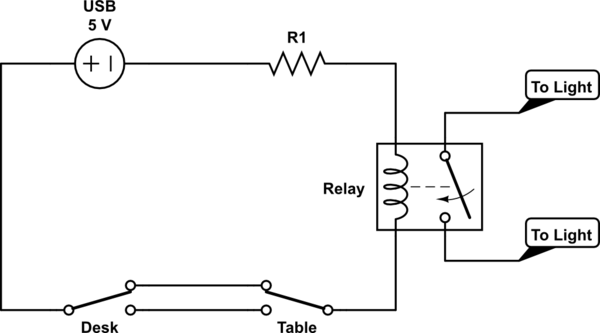
\includegraphics[width=.9\linewidth]{./relay.png}
\end{center}
Relays are literally coiled wires that creates electro-magnetic field when electricity goes through them. the magnetic field attracts the metalic wire, thus closes the circuit and the motor from Hollerith's Machine runs and does the calculation. But it was huge, had 3000+ relays and any mechanical thing is prone to wears-and-tears. You have to replace relays, If we consider average lifetime of a relay is 10years, even then you have to replace 120 relays everyday, which is impratical. Not to mention, there were other factors, like \texttt{Bugs}. So Grace Hopper said, \texttt{If there is a error with the computer, its caused by the bugs.} Thats where the word - bug - came from.\\
\begin{center}
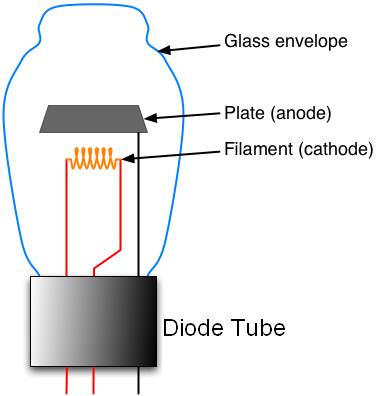
\includegraphics[width=.9\linewidth]{./vacumn-tube.png}
\end{center}

So we started looking for alternatives to mechanical relays and we found \texttt{Vacum Tubes} that was invented in 1904. This tube could replace relays. How it works?\\
When you heat a metal, it shoots out electrons. If we put +ve charge nearby, they complete a circuit! But if we give +ve charge to it, the nearby +ve wire deflects it and no circuit is formed. And thus, the motor can turn on and turn off!\\
And unlike mechanical relays, the Vacum Tube can turn on and tunr off 100s of times in a second so it increased computation efficiency hugely and not to mention, it does not wear down as fast as relays. So \texttt{Vacum Tubes} became the next standard.\\
But vacum tubes were big, they were fragile and so we found a new alternative - \texttt{Transistors!}. It used a semi-conductor to control the flow of electron and the size of Transistor kept decreasing. Its just 5 nanometer currently!\\

But how do we compute without using the old motors and gears? Thats what we will cover next episode.\\
\subsubsection*{Ep 4: Boolean Logic and Logic Gates}
\label{sec:orgde6b3cd}
Out previous method of calculation was - Moving gears. We later moved the gears using motor.\\
If electricity - move gears by one.\\
If no - dont move gears.\\

But soon, we noticed\\
\begin{itemize}
\item \texttt{Details in Note Khata}\\
\end{itemize}
\subsubsection*{Ep 5: Representing everything in Binary}
\label{sec:org0775b8b}
\begin{itemize}
\item Numbers \texttt{We know}\\
\item Floating Points  \texttt{Khata}\\
\begin{center}
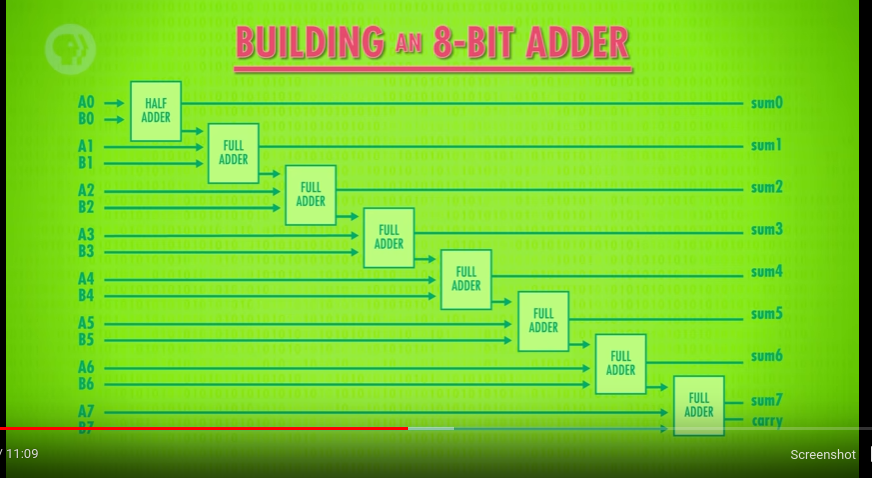
\includegraphics[width=.9\linewidth]{./addition-circuit.png}
\end{center}
\end{itemize}
\begin{itemize}
\item Characters - The trouble of Ascii
\label{sec:orgfcfd5b7}
First, We used 8 bit Ascii to represent characters. 8 bit = 256.\\
So we can represent at most 256 digits with it. So we did this back then -\\
256 = Language Characters + Mathematical Symbols + Scientific Symbols\\
e.g.  English + addition integral + alpha beta gama\\
e.g.  French + addition integral + alpha beta gama\\
But it soon create problem. As you guessed, there is no world wide standard. Each country has their own Symbols representation. As a result, a document written in english gives incomprehensible outcome when you open it in a French Computer.\\
Thats when UNICODE cam to our resque. Its 16bits long, meaning it can contain millions of unique characters. As a result, it contains every character of every language that has ever existed, emojis, scientific notations etc.\\
\end{itemize}
\subsubsection*{{\bfseries\sffamily TODO} Ep 6: How Computers Calculate}
\label{sec:org005643d}
\href{https://learnabout-electronics.org/Digital/dig58.php}{ALU Example}\\
\begin{center}
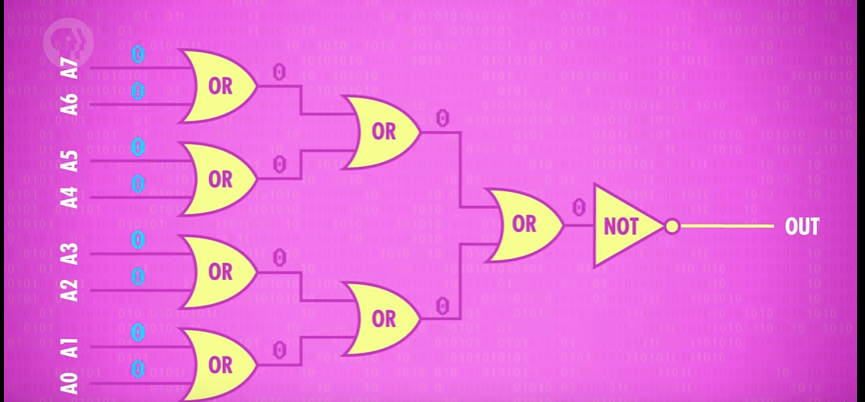
\includegraphics[width=.9\linewidth]{./ALU-check-number-equals-zero.png}
\end{center}
\begin{center}
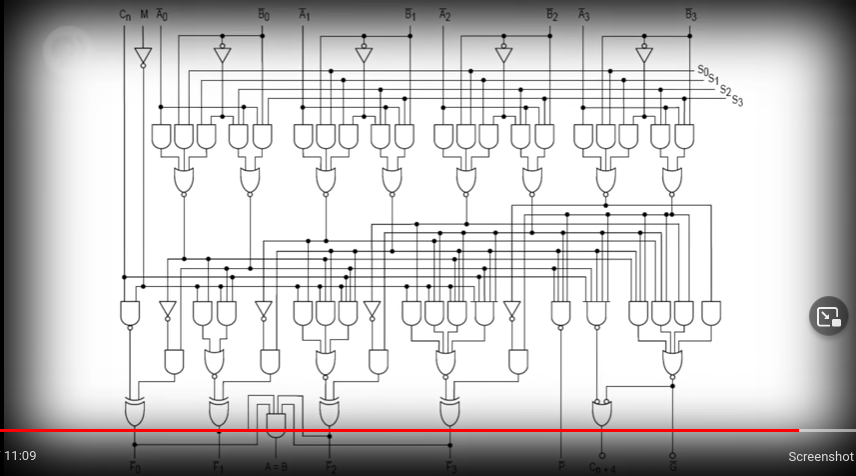
\includegraphics[width=.9\linewidth]{./ALU-made-of-logic-gates.png}
\end{center}
\url{./ALU-circuit.gif}\\
\subsubsection*{Ep 7: Registers and RAM}
\label{sec:org0a07116}
\begin{itemize}
\item Multiplexer\\
This far, we saw how to calculate using just transistors. But we need to store the results, input data somewhere to do more sophisticated operations.\\
\end{itemize}
Like fiding nth digit of fibonacci, we need to store two digits. So we need a memory.\\
\begin{itemize}
\item Memory Latch\\
\end{itemize}

As we saw, a latch can hold onto a single bit. If we put 8 such latches together, we can store 8 bits. Such collection of latches is called \texttt{Register}.(8 bit, 16 bit, 32bit, 64bit registers.)\\
\begin{itemize}
\item Algo to store data in register
\label{sec:orgfb7dc41}
\begin{itemize}
\item Set all latches' \texttt{Enable Write} bit to 1.\\
\item Now send the data to store to the latches. Like if we wish to store 00001101, then we will send 1 to latch0, 0 to latch1, 1 to latch2 etc.\\
\item Set \texttt{Enable Write} bit to 0 to save the data.\\
\end{itemize}

\begin{center}
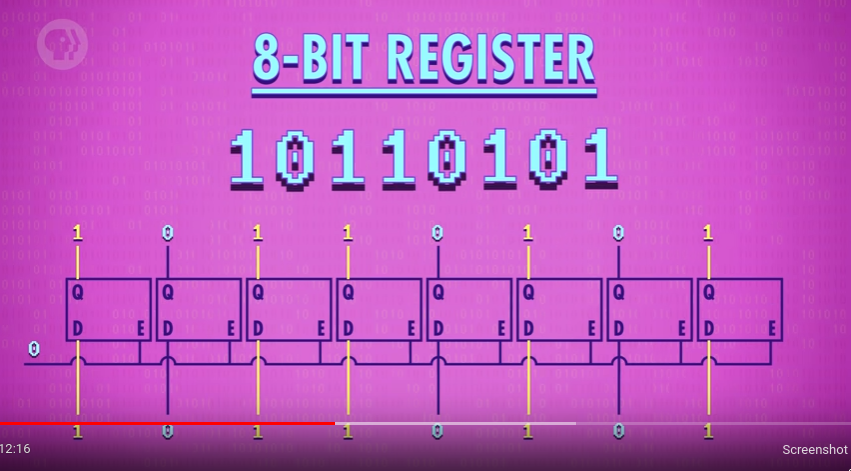
\includegraphics[width=.9\linewidth]{./saving-data-to-latch-register.png}
\end{center}

Poof,we just stored a 8 bit number into a register made of latches which are made of gates(transistors.)\\
\item The issue of Wiring cables and Latch Matrix
\label{sec:org81fe5c7}
As we saw in the picture, for a 8 bit register, we need 8 input wire, 8 output wire and 1 data wire.\\
Similarly, for 64 bit register, 64+64+1=129 wires.\\
Thats a lot of wires. So we use Latch Matrix.\\
\begin{center}
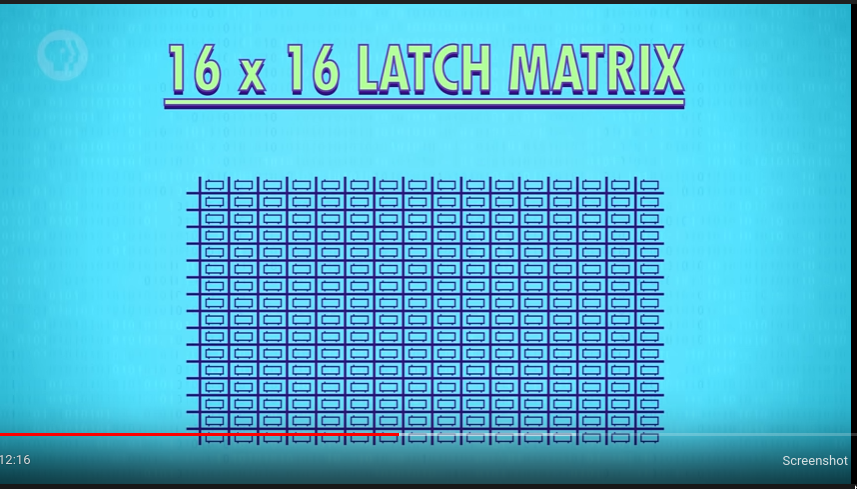
\includegraphics[width=.9\linewidth]{./latch-matrix.png}
\end{center}
\begin{center}
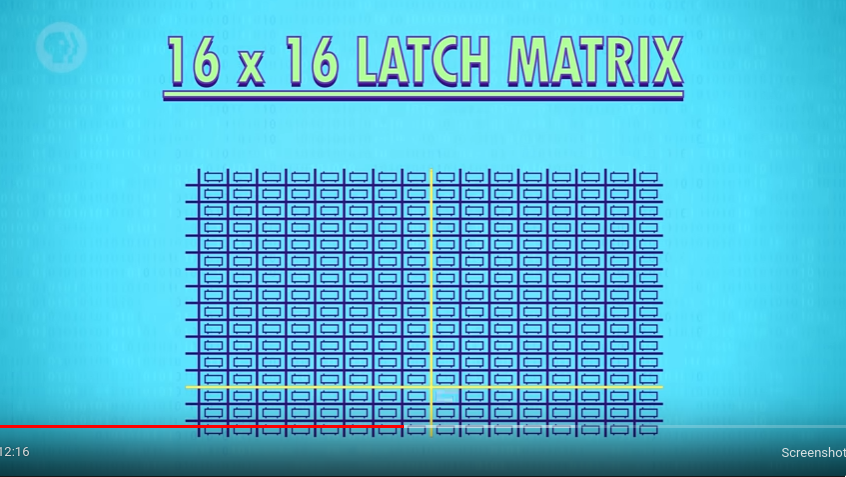
\includegraphics[width=.9\linewidth]{./latch-matrix-cell.png}
\end{center}
\begin{center}
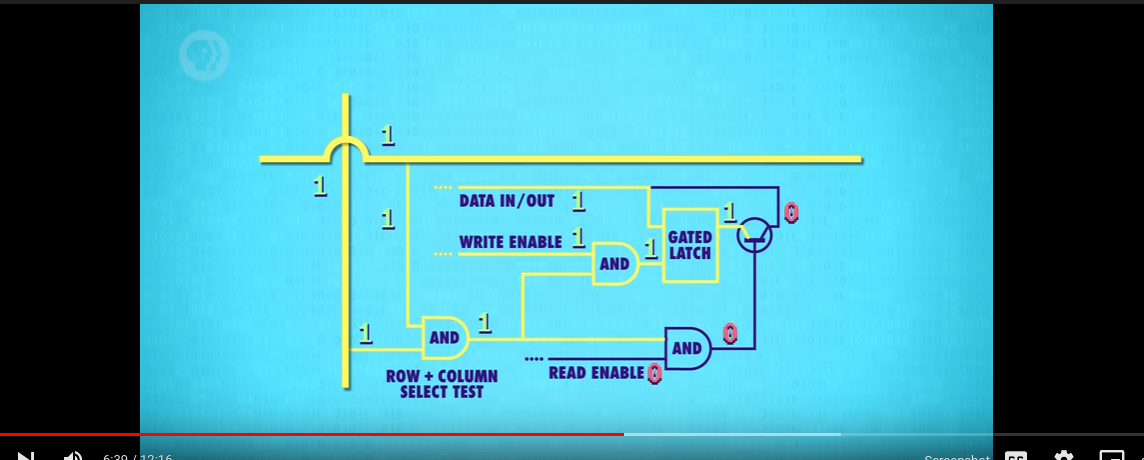
\includegraphics[width=.9\linewidth]{./latch-matrix-single-cell.png}
\end{center}

As we can uniquely select particular latch with latch-matrix row-column wires, we can just have a common data wire for all of the latches. Because at any given time, only one latch will be activated and take the data. Rest of the latches are not activated so will just ignore the data.\\

So for a 64 bit register, we need -\\
8+8+1 = 17 wires but we can store 64bit data!\\

But we need to be able to uniquely select the latch for that, like store data in latch(3,4). For that, we bring forth the idea of \texttt{Memory Address.}\\
\item Memory Address
\label{sec:org27a5c1a}
For row=12, column=10, we can make a memory address like -> 11001010\\
To convert from a address into being able to select exact latch, we use \texttt{Multiplexer.}\\
Lets work with 4->16 multiplexer.\\
\begin{itemize}
\item First, extract row and column portion of the memory addres.\\
\item Send the row portion to row multiplexer, column to column multiplexer, find the data, save it.\\
\end{itemize}
\begin{center}
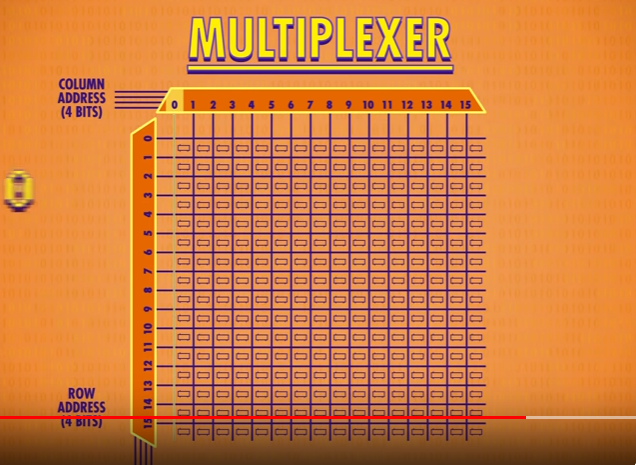
\includegraphics[width=.9\linewidth]{./multiplexer.png}
\end{center}
\item RAM
\label{sec:org3363014}
Lets abstract register.\\
\begin{center}
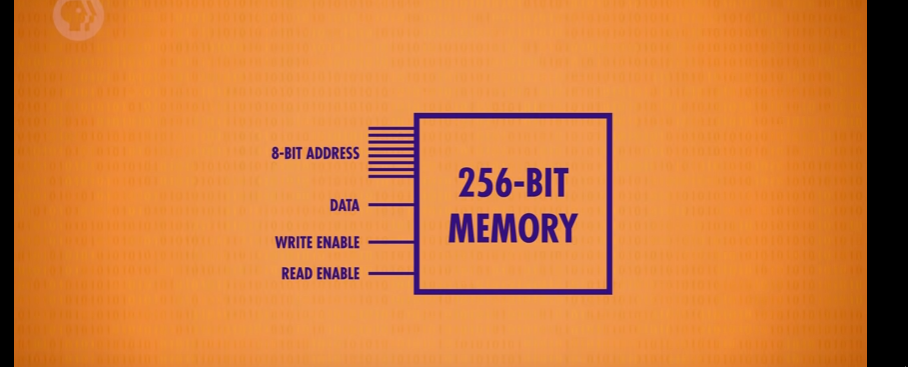
\includegraphics[width=.9\linewidth]{./register-abstraction.png}
\end{center}
But merely 256 bit data ain't much. So we line up multiple registers to store more data.\\
And poof, now we have RAM! RAM is volatile because data can only be stored as a loop and loop exists as long as there is current flowing through it.\\
\begin{center}
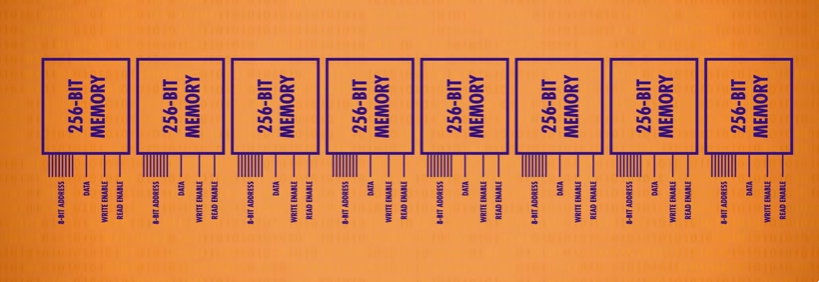
\includegraphics[width=.9\linewidth]{./ram.png}
\end{center}

Modern memories do the exact samething - package latches into small unit, then even smaller units, and even smaller units and so on.\\
\texttt{VIDEO(10:12-11)}\\
If we zoom in enough, we will see the matrix - 128X64 bits matrics. The video just is a 1MB RAM.(1980s) Remember that, we landed moon with 64kb RAM.\\
\end{itemize}
\subsubsection*{Ep 8: CPU}
\label{sec:orga1ca2f2}
\begin{itemize}
\item ALU + RAM\\
\end{itemize}
ALU can do arithmetic operations and simple logical operations.(like in mips). RAM can save the data. ALU was built using FA to do arithmetic operations, Simple circuits to check if a number is zero. RAM is built of latches in a matrix.\\

Remember mips. Our CPU Instructions were -> Save/Load Values, Arithmetic Operations, Conditions.\\

Now Lets see a CPU. \texttt{CPU IMAGE} We need two more things along with ALU and RAM for a CPU to function. Some register and a control unit.\\
Whats a control unit? Its the unit that will decide which instruction was sent. For example, If we send \texttt{1100} instruction to CPU, it has to first understand that its a comparison operation. So We need some simple gates to check which instruction was given. The following example shows a simple circuit that checks if the given instruction is LOAD\textsubscript{DATA}(0010).\\
\begin{center}
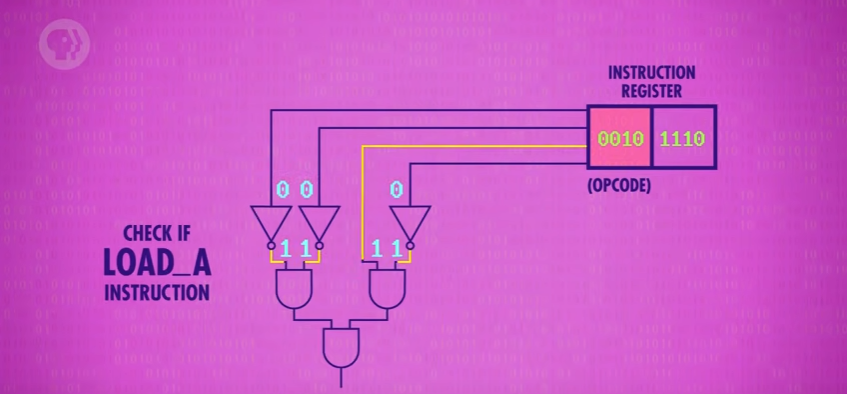
\includegraphics[width=.9\linewidth]{./control-unit-example.png}
\end{center}
So we have similar such simple gates to check the given instruction/opcode in the control unit.\\
\begin{center}
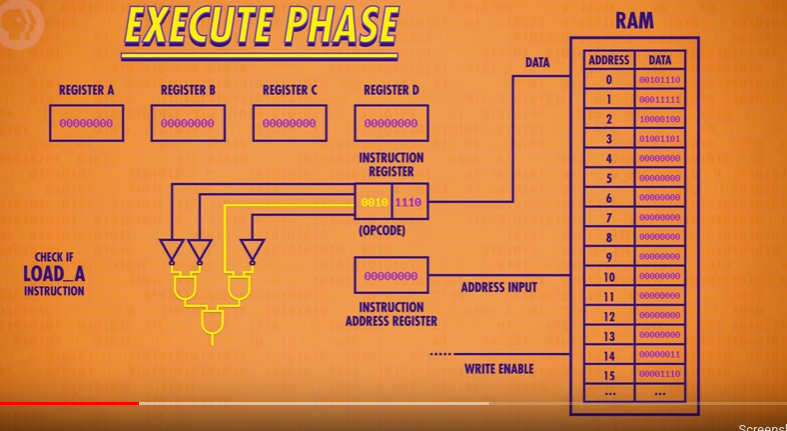
\includegraphics[width=.9\linewidth]{./cpu-with-bare-control-unit.png}
\end{center}

LOAD 12 in Register A\\
1100 00001100 00000001\\

We also need some register to hold current data, return address, next instruction address.\\

So CPU = RAM + control unit + Registers + ALU\\

First, when computer loads up, everything is empty.\\
\end{document}
